\documentclass{beamer}

\setlength{\parskip}{\baselineskip}
\setlength{\parindent}{0pt}
\usepackage{default}
\usepackage{tabularx}
\usepackage{url}
\usepackage{graphicx}

\title{\bf Handbook of Writing for the \\ Mathematical Sciences}
\author{Manuel Baumann, J\"orn Zimmerling}
\titlegraphic{ \vspace{-0.8cm}
   \includegraphics[scale=0.08]{images/TU_Delft_logo1.png}\hspace{4cm}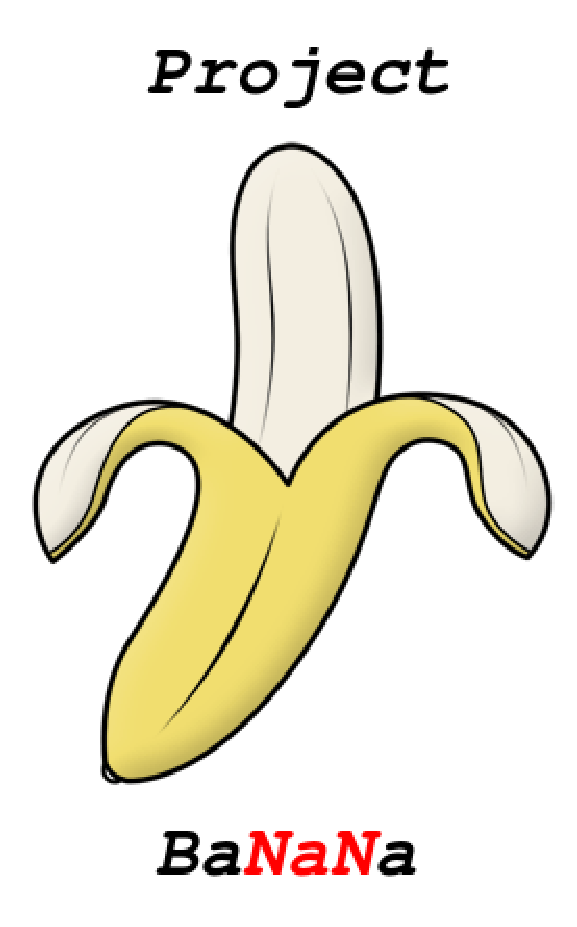
\includegraphics[scale=0.15]{../../images/logo}}
\date{\footnotesize{June 16, 2015}}
\begin{document}

\frame{\titlepage}
\begin{frame}
\frametitle{Handbook of Writing for the Mathematical Sciences}
\begin{columns}
 \begin{column}{0.6\textwidth}
I will present a ``best off'':

 \begin{itemize}
  \item Nicholas J. Higham. \emph{Handbook of Writing for the Mathematical Sciences, Second Edition,} 1998.
  \item high-level scientific writing
  \item for-and-by mathematicians
  \item highly \textit{pedantic}
 \end{itemize}
 \end{column}

 \begin{column}{0.4\textwidth}
  \begin{figure}[t]
  \centering
  \includegraphics[width=0.8\textwidth]{images/book_cover.jpg}
  \end{figure}
 \end{column}
 \end{columns}
 
\end{frame}

\begin{frame}
\frametitle{Did you know that ..?}
Q: Which one is correct?
\\
\begin{center}
 We use {\color{red}a/an} LAPACK routine.
\end{center}
{\color{white}A: The abbreviation reads ``ell-a-pack''.}
\end{frame}

\begin{frame}[noframenumbering]
\frametitle{Did you know that ..?}
Q: Which one is correct?
\\
\begin{center}
 We use {\color{red}an} LAPACK routine.
\end{center}
A: The abbreviation reads ``ell-a-pack''.
\end{frame}

\begin{frame}
 \tableofcontents
\end{frame}

\section{Scientific writing}
\begin{frame}
\frametitle{Scientific writing (1/3)}
\begin{figure}[t]
 \includegraphics[width=0.9\textwidth]{images/ten.jpeg}
\end{figure}
\end{frame}
\begin{frame}
\frametitle{Scientific writing (2/3)}
% \begin{figure}[t]
%  \includegraphics[width=0.8\textwidth]{images/ten.jpeg}
% \end{figure}
\end{frame}
\begin{frame}
\frametitle{Scientific writing (3/3)}
% \begin{figure}[t]
%  \includegraphics[width=0.8\textwidth]{images/ten.jpeg}
% \end{figure}
\end{frame}

\section{Mathematical expressions}
\begin{frame}
\frametitle{Mathematical expressions (1/5)}
\begin{figure}[t]
 \includegraphics[width=\textwidth]{images/punct.jpeg}
\end{figure}
\end{frame}
\begin{frame}
\frametitle{Mathematical expressions (2/5)}
% \begin{figure}[t]
%  \includegraphics[width=0.8\textwidth]{images/punct.jpeg}
% \end{figure}
\end{frame}
\begin{frame}
\frametitle{Mathematical expressions (3/5)}
% \begin{figure}[t]
%  \includegraphics[width=0.8\textwidth]{images/punct.jpeg}
% \end{figure}
\end{frame}
\begin{frame}
\frametitle{Mathematical expressions (4/5)}
% \begin{figure}[t]
%  \includegraphics[width=0.8\textwidth]{images/punct.jpeg}
% \end{figure}
\end{frame}
\begin{frame}
\frametitle{Mathematical expressions (5/5)}
% \begin{figure}[t]
%  \includegraphics[width=0.8\textwidth]{images/punct.jpeg}
% \end{figure}
\end{frame}


\section{High-end \LaTeX}
\begin{frame}
\frametitle{High-end \LaTeX (1/3)}
% \begin{figure}[t]
%  \includegraphics[width=0.8\textwidth]{images/punct.jpeg}
% \end{figure}
\end{frame}
\begin{frame}
\frametitle{High-end \LaTeX (2/3)}
% \begin{figure}[t]
%  \includegraphics[width=0.8\textwidth]{images/punct.jpeg}
% \end{figure}
\end{frame}
\begin{frame}
\frametitle{High-end \LaTeX (3/3)}
% \begin{figure}[t]
%  \includegraphics[width=0.8\textwidth]{images/punct.jpeg}
% \end{figure}
\end{frame}


\section{BE vs. AE}
\begin{frame}
\frametitle{BE vs. AE (1/2)}
% \begin{figure}[t]
%  \includegraphics[width=0.8\textwidth]{images/punct.jpeg}
% \end{figure}
\end{frame}
\begin{frame}
\frametitle{BE vs. AE (2/2)}
% \begin{figure}[t]
%  \includegraphics[width=0.8\textwidth]{images/punct.jpeg}
% \end{figure}
\end{frame}


\section{Miscellaneous}
\begin{frame}
\frametitle{Miscellaneous (1/4)}
% \begin{figure}[t]
%  \includegraphics[width=0.8\textwidth]{images/punct.jpeg}
% \end{figure}
\end{frame}
\begin{frame}
\frametitle{Miscellaneous (2/4)}
% \begin{figure}[t]
%  \includegraphics[width=0.8\textwidth]{images/punct.jpeg}
% \end{figure}
\end{frame}\begin{frame}
\frametitle{Miscellaneous (3/4)}
% \begin{figure}[t]
%  \includegraphics[width=0.8\textwidth]{images/punct.jpeg}
% \end{figure}
\end{frame}
\begin{frame}
\frametitle{Miscellaneous (4/4)}
% \begin{figure}[t]
%  \includegraphics[width=0.8\textwidth]{images/punct.jpeg}
% \end{figure}
\end{frame}

\begin{frame}
\frametitle{Further reading}
Many information are available online:
\begin{itemize}
 \item \url{https://github.com/}
 \item \url{http://try.github.io/levels/1/challenges/1}
 \item \url{http://git-scm.com/book}
\end{itemize}
These slides, and much more, will \textit{not} be published at:
\begin{itemize}
 \item \url{http://projectbanana.github.io/}
\end{itemize}
 \begin{figure}
\centering
 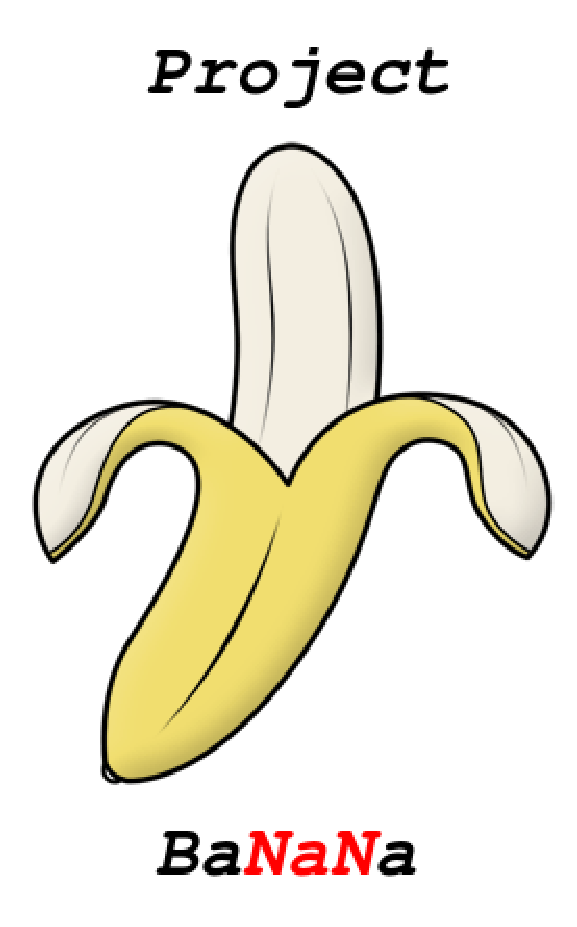
\includegraphics[height=0.3\textheight]{../../images/logo}
\end{figure}
\end{frame}

\end{document}
